\documentclass{beamer}
\usepackage[utf8]{inputenc}
\usepackage[T1]{fontenc}
\usepackage{tikz}
\usetikzlibrary{shapes.geometric}
\usepackage{standalone}
\usepackage{amsmath}
\usepackage{amsfonts}
\usepackage{graphicx, color}
\usepackage{svg}

\newcommand{\E}{\mathbb{E}}
\newcommand{\Norm}{\mathcal{N}}
\newcommand{\Loss}{\mathcal{L}}
\newcommand{\R}{\mathbb{R}}
\newcommand{\bt}{\mathbf{t}}
\newcommand{\bU}{\mathbb{U}}
\newcommand{\bu}{\mathbf{u}}
\newcommand{\bw}{\mathbf{w}}
\newcommand{\bX}{\mathbf{X}}
\newcommand{\bx}{\mathbf{x}}
\newcommand{\by}{\mathbf{y}}
\newcommand{\bZ}{\mathbf{Z}}
\newcommand{\bz}{\mathbf{z}}

\newcommand{\eq}{=}
\newcommand{\parfrac}[2]{\frac{\partial #1}{\partial#2}}

\title{Causal Effect Inference with Normalising Flows}
\author{Micha de Groot}


\begin{document}
	
	\begin{frame}
		\titlepage
	\end{frame}
	
	
	\begin{frame}{New dataset} 
		\begin{figure}
            \centering
            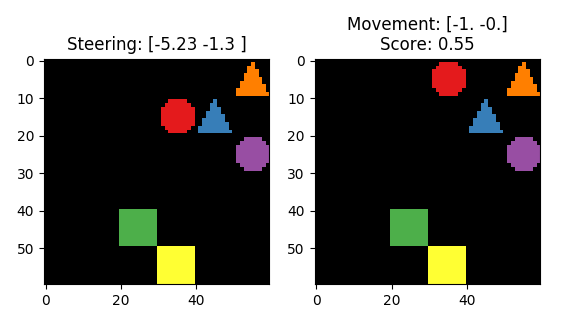
\includegraphics[scale=0.7]{latex/Figures/sample_space_shapes_with_score.png}
            \caption{Sample of the dataset. Image on the left is the proxy variable $\bx$, Steering on the left is the intervention variable $\bt$, score on the right is the outcome variable $\by$. Image and direction vector on the right is a visualisation of what 'happens' because of the confounding combined with the intervention variable.}
            \label{fig:graph_observed_confounder_and_latent_with_proxy}
        \end{figure}
	\end{frame}
	
	\begin{frame}{Some considerations I made}
		\begin{itemize}
		    \item Keep the outcome variable $\by$ a vector or scalar. Having the possibility of it also being an image itself might deviate a bit too much from earlier work where it is always just a scalar and it makes the code a lot more cumbersome because it needs to take more model options into account.
		    \item For now more noise to all variables is optional and can be scaled up after adding the technical novelty is done.
		    \item The causal flow model I designed needs major improvement or we need to come up with something different altogether. 
		\end{itemize}
	\end{frame}
	
	\begin{frame}{Causal flow model and its problems}
	    The model is based on the RealNVP. In the RealNVP we have invertible coupling layers:
	    \begin{align}
	        \bz_{k+1, 1:d} &= \bz_{k, 1:d} \\
            \bz_{k+1, d+1:D} &= \bz_{k, d+1:D} \odot \exp \left(s(\bz_{k, 1:d}) \right) + t(\bz_{k, 1:d})
	    \end{align}
	    Each layer half of the dimensions is translated and scaled, based on a NN that takes the other half as input, meaning $s(\cdot)$ and $t(\cdot)$ are arbitrary neural networks.
	\end{frame}
	
	\begin{frame}{Causal flow model and its problems}
	    The idea was to use three of these chains of coupling layers. The first one maps the proxy variable $\bx$ to an intermediate representation $\bx_k$. The second one maps the outcome variable $\by$ to an intermediate representation $\by_k$. And for the third one we concatenate $\bx_k$ and $\by_k$ and pass that through the coupling layers to get $\bz$.
	    
	    We use the intervention variable $\bt$ as 'context' in the series of coupling layers from $\by$ to $\by_k$. This means that $\bt$ is given as additional input to the networks $s(\cdot)$ and $t(\cdot)$ in each coupling layer between $\by$ and $\by_k$.
	\end{frame}
	
	\begin{frame}{Causal flow model and its problems}
	     During test time we want to do two things: first infer $\bz$ based on $\bx$, and then set $\bt$ to a specific value and infer $\by$ from $\bz$ and $\bt$. The second part is straightforward with this model, but the first part isn't.
	     
	     The original CEVAE does this in three steps:
	     \begin{enumerate}
	         \item Predict and sample $\bt$ solely on $\bx$
	         \item Predict and sample $\by$ with $\bx$ and the new $\bt$ value
	         \item Predict and sample $\bz$ with $\bx$ and the new $\bt$ and $\by$ value
	     \end{enumerate}
	     The first two are done with separate networks that aren't really part of the CEVAE and are trained in a supervised way. We could also do this but it doesn't seem elegant. 
	\end{frame}
	
	\begin{frame}{Causal flow model and its problems}
	    I tried to avoid the partial supervised approach in the following way. Instead of predicting $\by$ and $\bt$ from $\bx$, and then using those to predict $\bz$ I selected an array of $n$ evenly spaced values for both $\by$ and $\bt$ within their respective range. The range was determined by taking the min and max of the training data.
	    Then I took all combinations of $\bt$ and $\by$ values, combined them with $\bx$ and passed them through the coupling layers. This yields a set of $n$ $\bz$ values, which I averaged. 
	    Then that $\bz$ value was passed through the reverse of the flow, combined with the value of $\bt$ for which we actually wanted to predict the outcome, to make our final prediction of $\by$.
	\end{frame}
	
	\begin{frame}{Causal flow model and its problems}
	    Another problem with the RealNVP-based approach is that if $\by$ is low dimensional the coupling layers are less powerful, since each scaling and translation network has a low dimensional input. It was designed for high dimensional images.
	\end{frame}
	
\end{document}